% This is based on the LLNCS.DEM the demonstration file of
% the LaTeX macro package from Springer-Verlag
% for Lecture Notes in Computer Science,
% version 2.4 for LaTeX2e as of 16. April 2010
%
% See http://www.springer.com/computer/lncs/lncs+authors?SGWID=0-40209-0-0-0
% for the full guidelines.
%
\documentclass{llncs}

\usepackage{hyperref}
\usepackage{xspace}
\usepackage{graphicx}
\usepackage{amsmath}
\usepackage{amssymb}
\usepackage{url}
\usepackage{booktabs}
\usepackage{makecell}
\usepackage[usenames, dvipsnames]{color}


%% Use this during review mode
%\usepackage{review}
%% Use this for final compiling
\usepackage[final]{review}


\pagestyle{headings} 


\hyphenation{Zstandard}


\begin{document}


% Name of our compression tool. This is subject to change ;)
\newcommand{\appName}{Compresso\xspace}
\newcommand{\appUrl}{\url{https://github.com/Rhoana/bockwurst}}
\newcommand{\squeezeup}{\vspace{-10mm}}
\newcommand{\shspace}{\vspace{-5mm}}

\newcommand{\floatfootnote}[1]{\ifx\[$\else\footnote{#1}\fi}

\title{\appName: Efficient Compression of Segmentation Data For Connectomics}
%
\titlerunning{\appName: Compression of Segmentation Data}  % abbreviated title (for running head)
%                                     also used for the TOC unless
%                                     \toctitle is used
%
\author{Brian Matejek, Daniel Haehn, Fritz Lekschas, Michael Mitzenmacher, Hanspeter Pfister}
% index{Matejek, Brian}
% index{Haehn, Daniel}
% index{Lekschas, Fritz}
% index{Mitzenmacher, Michael}
% index{Pfister, Hanspeter}	
%
%\authorrunning{Brian Matejek et al.} % abbreviated author list (for running head)
%
%%%% list of authors for the TOC (use if author list has to be modified)
\tocauthor{}
%
\institute{Harvard University, Cambridge, MA 02138, USA\\
\email{bmatejek,haehn,lekschas,michaelm,pfister@seas.harvard.edu}}

\maketitle              % typeset the title of the contribution

\shspace
\begin{abstract}
Recent advances in segmentation methods for connectomics and biomedical imaging produce very large datasets with labels that assign object classes to image pixels. The resulting label volumes are bigger than the raw image data and need compression for efficient storage and transfer. General-purpose compression methods are less effective because the label data consists of large low-frequency regions with structured boundaries unlike natural image data. We present \appName, a new compression scheme for label data that outperforms existing approaches by using a sliding window to exploit redundancy across border regions in 2D and 3D. We compare our method to existing compression schemes and provide a detailed evaluation on eleven biomedical and image segmentation datasets. Our method provides a factor of 600-2200x compression for label volumes, with running times suitable for practice.

\keywords{compression, encoding, segmentation, connectomics}
\end{abstract}
\shspace

%

\section{Introduction} \label{sec:i}

Connectomics---reconstructing the wiring diagram of a mammalian brain at nanometer resolution---results in datasets at the scale of petabytes~\cite{haehn_dojo_2014,suissapeleg2016}. Machine learning methods find cell membranes and create cell body labelings for every neuron~\cite{liu2014modular,GALA2014,ronneberger2015u} (Fig.~\ref{fig:data}).
%aims to reconstruct the wiring diagram of a mammalian brain at nanometer resolution. This results in datasets at the scale of petabytes~\cite{suissapeleg2016}. 
%These shear amounts of data require sophisticated methods of compression to enable efficient storage and transfer. 
These segmentations are stored as label volumes that are typically encoded in 32 bits or 64 bits per voxel to support labeling of millions of different nerve cells (neurons).  Storing such data is expensive and transferring the data is slow. To cut costs and delays, we need compression methods to reduce data sizes.

%Our work stems from a collaboration between computer scientists and neuroscientists in the field of connectomics. 
%Connectomics aims to reconstruct the wiring diagram of a mammalian brain at nanometer resolution, comprising millions of nerve cells (neurons) and their interconnections. 
%By deciphering this vast network and analyzing its underlying properties, scientists hope to better understand mental illnesses, learning disorders, and neural pathologies.

\begin{figure}[h]
	\begin{center}
		
\includegraphics[width=0.38\textwidth]{gfx/ac3.png}%
		\hspace{0.12\textwidth}
		
\includegraphics[width=0.38\textwidth]{gfx/cyl.png}%
	\end{center}
\caption{Examples of connectomics segmentation data with a different color per cell.}
\label{fig:data}
\end{figure}

%To analyze neuronal connectivity at the level of individual connections of neurons, we acquire and process high-resolution electron microscopy (EM) image stacks. 
%Recent progress in automatic sample preparation and EM acquisition techniques increases these datasets to petabytes in size~\cite{suissapeleg2016}.
%Machine learning methods find cell membranes and create cell body labelings for every neuron~\cite{ronneberger2015u,liu2014modular,GALA2014} (Fig.~\ref{fig:data}). 
%These segmentations are stored as label volumes, which are typically encoded in 32 bits or 64 bits per voxel to support millions of unique labels. 
%Storing such data is costly, and transferring the data is slow. To cut costs and delays, we need compression methods to reduce data sizes.

%One approach to allow data analysis of these volumes is to pre-process the segmentation data and store it uncompressed as a tiled quadtree data structure on a network filesystem.
%Researchers then access the segmentation data with thin clients, e.g., web-based applications like Dojo~\cite{haehn_dojo_2014}.
%The quadtree structure represents different pre-computed zoom levels of the data and enables loading and exploration of downsampled images.
%This scenario imposes three problems: offline storage, data transmission, and random access.
%Currently, the complete dataset is stored on disk and only a subset is transferred depending on individual use cases. This works well; however, recent progress in automatic sample preparation and EM acquisition techniques increases connectomics data to terabytes in size~\cite{RonnebergerFB15,GALA2014}. Storage and transmission of such massive datasets is hard and expensive, and access can be slow. Therefore, we need compression methods to reduce data sizes.

The literature currently lacks efficient compression of label volumes. 
General-purpose compression schemes~\cite{collet2016smaller,deutsch1996zlib,google2016brotli,lehmann2016liblzf,oberhumer2005lzo,pavlov2007lzma,seward1998bzip2,vandevenne2016zopfli,welch1984technique,ziv1978compression} are not optimized for this data.
In this paper, we exploit the typical characteristics of label volumes such as large invariant regions without natural relationship between label values. 
These properties render 2D image compression schemes inadequate since they rely on frequency reduction (using e.g., wavelet or discrete cosine transform) and value prediction of pixels based on local context (differential pulse-code modulation)~\cite{roelofs1999png,skodras2001jpeg}. 
Color space optimization strategies in video codecs~\cite{aimar2005x264} also have no effect on label volumes, even though the spatial properties of a segmentation stack (\textit{z}-axis) are similar to the temporal properties of video data (time-axis). 
A compression scheme designed specifically for label volumes is part of the visualization software Neuroglancer~\cite{google2016compressed}. 
This method exploits segmentation homogeneity by creating small blocks with $N$ labels and reducing local entropy to $\log_2{N}$ per pixel. 
Lookup tables then decode the values $[0,N)$ to the original 64-bit labels. We compare the Neuroglancer scheme with our method.
%The most relevant current compression tool is Neuroglancer~\cite{google2016compressed}---a web-based 3D segmentation viewer that provides a compression scheme for segmentation data.
%
%The assumption behind this scheme is that, on average, small local areas will contain very few unique labels with high probability. Based on this assumption, Neuroglancer divides the segmentation data into several small blocks. Pixels inside a block with $N$ distinct labels only require $\log_2{N}$ bits of information to encode.
%
%A lookup table for each block maps the values $[0, N)$ to the original 64-bit label. We compare the performance of Neuroglancer with our scheme in Sec.~\ref{sec:results}.
%
%A compression scheme for labeled volumes is part of the 3D segmentation viewer Neuroglancer~\cite{google2016compressed}. This method exploits segmentation homogeneity by creating small blocks with $N$ labels, reducing entropy to $\log_2{N}$. Lookup tables map the values $[0,N)$ to the original 64-bit labels. We compare the performance of Neuroglancer with our scheme in Sec.~\ref{sec:results}.
%
%and therefor reduces the
%to exploit homogeneity
%
%The most relevant current compression is

We explore the lossless compression of gigavoxel neuron segmentation volumes with high bit-encodings. 
We study and evaluate the performance of existing lossless compression methods, and their combinations, on multiple connectomics, magnetic resonance imaging (MRI) and general segmentation datasets.
As our main contribution, we present \appName---a novel compression method designed for label volumes using windowed feature extraction. 
\appName yields compression ratios on label volumes 80\% higher than the current best tools (Sec.~\ref{sec:results}).
We release an open-source C++ implementation of our method including a Python interface.


%\section{Related Work} \label{sec:rl}
%
%\paragraph{Data Storage.}
%For data storage we are mostly interested in compression tools with compression rates.
%There are many studies~\cite{alakuijala2015comparison,squash2016squash,mahoney2016large,lzturbo2016lzturbo,turbobench2016turbobench} evaluating general compression tools in regards to their compression rate, compression speed, and decompression speed.
%Classic encoders are zlib~\cite{deutsch1996zlib} (which utilizes LZ77~\cite{ziv1977universal}, LZ78~\cite{ziv1978compression}, LZF~\cite{lehmann2016liblzf}, LZO~\cite{oberhumer2005lzo}, LZW~\cite{welch1984technique}, and Huffmann codes~\cite{huffman1952method}), bzip2 (using run-length encoding, the Burrows-Wheeler transformation~\cite{burrows1994block}, move-to-front encoding, and delta encoding), and LZMA; LZMA is usually reported to provide best compression rates.
%
%\paragraph{Data Transmission.}
%
%Since major browsers natively support Zlib-based decompression, this method is predominantly used for concise data transmission from server to client. All major 
%
%Generally, there are two important aspects for data transmission: the size of the data being transferred and the time it takes to decompress that data.
%
%The first aspected is important as outwards traffic is expensive while the second aspect takes the overall response time into account.
%Zopfli~\cite{vandevenne2016zopfli} provides zlib compatible data streams with a slightly higher compression rate at the expense of a dramatically increased compression time.
%Another tool, recently published by Google, is Brotli~\cite{google2016brotli}---an LZ77-based compression tools that provides comparable compression rates to bzip2 at slow compression speed but high decompression speed.
%Finally, Facebook released Zstandard~\cite{collet2016smaller}, which claims to provide faster speeds and higher ratios.

\paragraph{General-purpose Compression.} Compression tools are well studied and compared in regards to their compression rate, compression speed, and decompression speed~\cite{alakuijala2015comparison,squash2016squash,mahoney2016large,lzturbo2016lzturbo,turbobench2016turbobench}. Classic encoders are zlib~\cite{deutsch1996zlib} (which utilizes LZ77~\cite{ziv1977universal} and Huffmann codes~\cite{huffman1952method}), LZ78~\cite{ziv1978compression}, LZF~\cite{lehmann2016liblzf}, LZO~\cite{oberhumer2005lzo}, LZW~\cite{welch1984technique}, bzip2~\cite{alakuijala2015comparison},
% (using run-length encoding, the Burrows-Wheeler transformation~\cite{burrows1994block}, move-to-front encoding, and delta encoding), 
and LZMA; LZMA is usually reported to provide very high compression rates.% which we observe also in our experiments. 
Recent efforts to optimize these approaches include Zopfli~\cite{vandevenne2016zopfli}, Brotli~\cite{google2016brotli}, and Zstandard~\cite{collet2016smaller}.

% Several efforts tried to optimize these approaches, such as Zopfli~\cite{vandevenne2016zopfli}, which provides zlib compatible data streams with a slightly higher compression rate at the expense of an increased compression time. Another optimization, recently published by Google, is Brotli~\cite{google2016brotli}---an LZ77-based compression tools that provides comparable compression rates to bzip2 with high decompression speed. Finally, Facebook released Zstandard~\cite{collet2016smaller}, which claims to provide faster speeds and higher ratios. 

All general-purpose methods are targeted towards handling any kind of data and we evaluate a variety on our datasets, resulting in compression without exploiting the typical characteristics of segmentation data. In addition, some methods are not able to handle the size of our datasets (Sec. \ref{sec:results}).

\paragraph{Image Compression.}
Many compression schemes for 2D images exist. The two most prominent lossless compression methods are PNG and JPEG2000 --- optimized for photographs. These techniques rely on frequency reduction (using e.g., wavelet or discrete cosine transform) and value prediction of images based on local context (differential pulse-code modulation). In contrast to photographs, segmentation data consists of large invariant regions and no natural relationship between their identifiers.

The typical frequency reductions and value predictions can not be applied to segmentation data. Therefore, off-the-shelf image compression techniques are not optimized and provide lower compression ratios. We still include PNG and JPEG2000 for evaluation.

\paragraph{Video Compression.} 
The \textit{z}-axis of a segmentation stack can be mapped to the time axis of video data. This relates video compression to segmentation compression. In practice, the change between slices in connectomics segmentation data is limited given natural constraints of the shape of cell bodies and restrictions in between-slice resolution. 
%There is a variety of different lossless compression tools for videos.

The currently most widespread video compression is x264 which provides lossless encoding when quantization is disabled. Intuitively, this does not yield the best performance on segmentation data, since any possible color space optimization is not applicable. 
Nevertheless, we include x264 for evaluation in Sec.~\ref{sec:results}.

\paragraph{Neuroglancer.} 
% \subsection{Neuroglancer} \label{sec:rl:neuroglancer}
The closest current compression tool is Neuroglancer~\cite{google2016compressed}---a web-based 3D segmentation viewer that provides a compression scheme for segmentation data. 
The assumption behind the compression scheme is that, on average, small local areas will contain very few distinct segment identifiers with high probability. 
Based on this assumption, Neuroglancer divides the segmentation data into several small blocks. 
Consider an arbitrary block $b$ with $N$ distinct segment identifiers.
Neuroglancer maps the identifier for each pixel into $[0, N)$ and stores a lookup table for $[0, N)$ to the original value. 
This reduces the number of bits needed to encode a pixel in a given block to $\log_2{N}$. 
The lookup table requires $64 * N$ bits of information to reconstruct the original data. 
In order to allow random access, Neuroglancer creates a header that stores the byte offset to the lookup table and encoded values for each block.
We compare the performance of Neuroglancer with our scheme in Sec. \ref{sec:results}.


\section{The \appName Scheme} \label{sec:m}

\subsection{Encoding}

\paragraph{Overview.}

Segmentation datasets contain two important pieces of information across the image stack: per-segment shape and per-pixel label. 
Decoupling these two components allows for better compression on each.

\paragraph{Boundary Encoding.}
\label{sec:boundary-map}

To encode the segment shapes, we consider the boundary pixels between two segments. 
Removing the per-pixel labels, we produce a boundary map for each slice where a pixel $(x, y, z)$ is 1 if either pixel at $(x + 1, y, z)$ or $(x, y + 1, z)$ belongs to a different segment. 
The boundary map is divided into non-overlapping congruent 3D windows. If there are $n$ pixels per window, each window $w$ is assigned an integer $V_w \in [0, 2^n)$ where $V_w$ is defined as:

\begin{equation}
V_w = \sum_{i = 0}^{n - 1} \mathbb{I}(i) 2^i,
\end{equation}

\noindent
and $\mathbb{I}(i)$ is 1 if pixel $i$ is on a boundary and 0 otherwise. 
Figure~\ref{fig:bockwurst-encoding} shows an example segmentation with a window size of $4 \times 4 \times 1$.

\begin{figure}[h]
  \begin{center}
    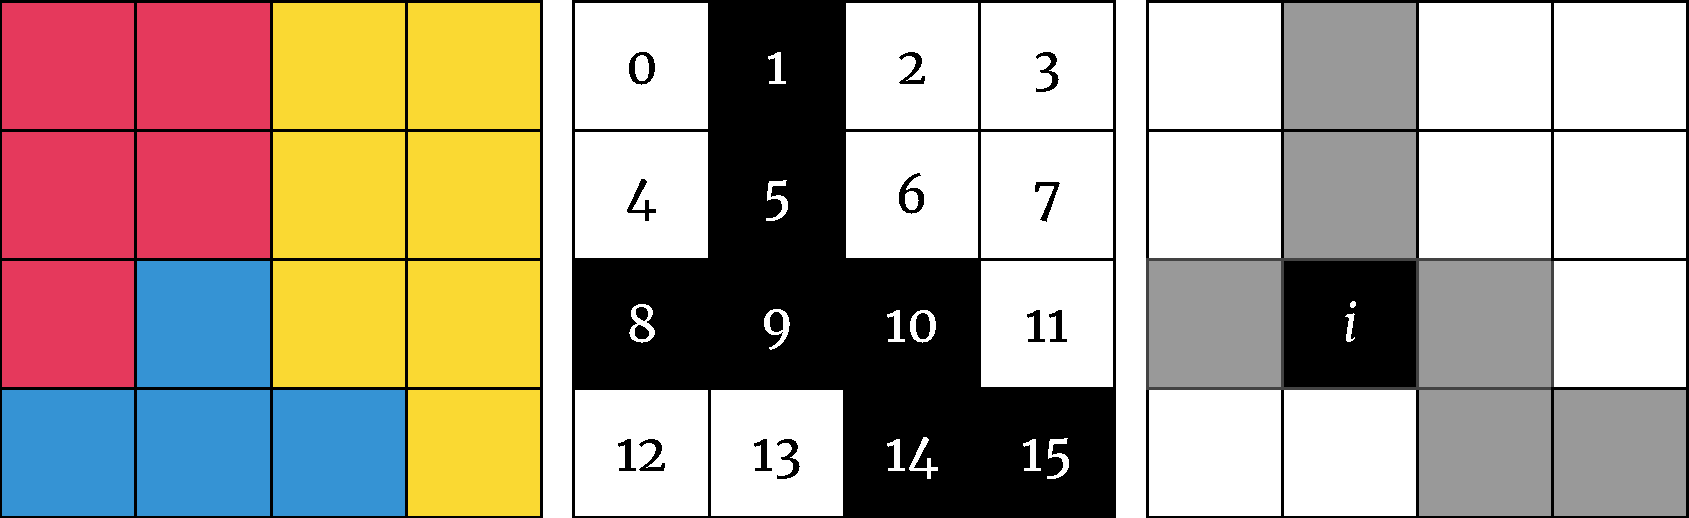
\includegraphics[width=0.7\textwidth]{gfx/encoding_diagram_opt.pdf}
  \end{center}
  \caption{A $4 \times 4 \times 1$ pixel window where three unique labels meet (left). The boundary map for the same window, where dark pixels represent the boundary (center). This window has an encoded value of 50,978 $(2^1 + 2^5 + 2^8 + 2^9 + 2^{10} + 2^{14} + 2^{15})$. A boundary pixel $i$ that is indeterminate and requires additional decoding information (right).}
  \label{fig:bockwurst-encoding}
\end{figure}

A priori, each window could take any of $2^n$ distinct values, and therefore require $n$ bits to encode without further manipulation. 
However, boundaries in segmentation images are not random, and many of these values never appear. 
Indeed, we find that a small subset of high-frequency $V_w$ values accounts for most windows, allowing for significant compression. 
Figure~\ref{fig:bockwurst-frequency} shows the 100 most common windows for a representative connectomics dataset. 
These 100 frequently occurring windows account for approximately 82\% of the over 1.2 million $V_w$ values in this dataset.
Nearly all of these windows correspond to simple lines traversing through the window. 
For contrast, we also provide 5 randomly generated windows that never occur in the dataset.

We define $N$ as the number of distinct $V_w$ representing all of the windows in an image stack. 
We construct an invertible function $f(V_w) \to [0, N)$ to transform the window values into a smaller set of integers. 
For all real-world segmentations $N \ll 2^n$; however, we assume no constraint on $N$ in order to guarantee lossless compression. 
With this function, each $V_w$ requires $\log_2{N}$ bits of information to encode. 
This is fewer than the initial number of bits so long as $N \leq 2^{n - 1}$.  
We create two arrays that store the per-segment shape encoding: $\texttt{WindowValues[]}$ contains the value $f(V_w)$ for every window $w$ and $\texttt{ValueMapping[]}$ contains the reverse mapping from $[0, N) \to [0, 2^n)$ based on the function $f$. 
Long sequences of $0$s in $\texttt{WindowValues[]}$ are reduced using run-length encoding.
%\vspace{-1mm}
\paragraph{Per-Pixel Label Compression.}

So far we have focused exclusively on transforming the boundary map of an image segmentation. 
However, the per-pixel labels themselves are equally important. 
The boundary map divides each image slice into different segments. 
By design, all pixels in the same segment have the same label so we store only one label per segment for each slice. 
We use a connected-component labeling algorithm to store one label per segment \cite{he2009fast}. 
The algorithm labels all pixels clustered within a component $m$ from $M$ section labels.
We store the original label for a segment $m$ in slice $z$ in $\texttt{Labels}_z\texttt{[m]}$. 
We concatenate these arrays for every image slice to create a variable $\texttt{Labels[]}$.
%\vspace{-1mm}
\paragraph{Exceptions.}

\begin{figure}
  \begin{center}
    \begin{minipage}{.8\linewidth}
      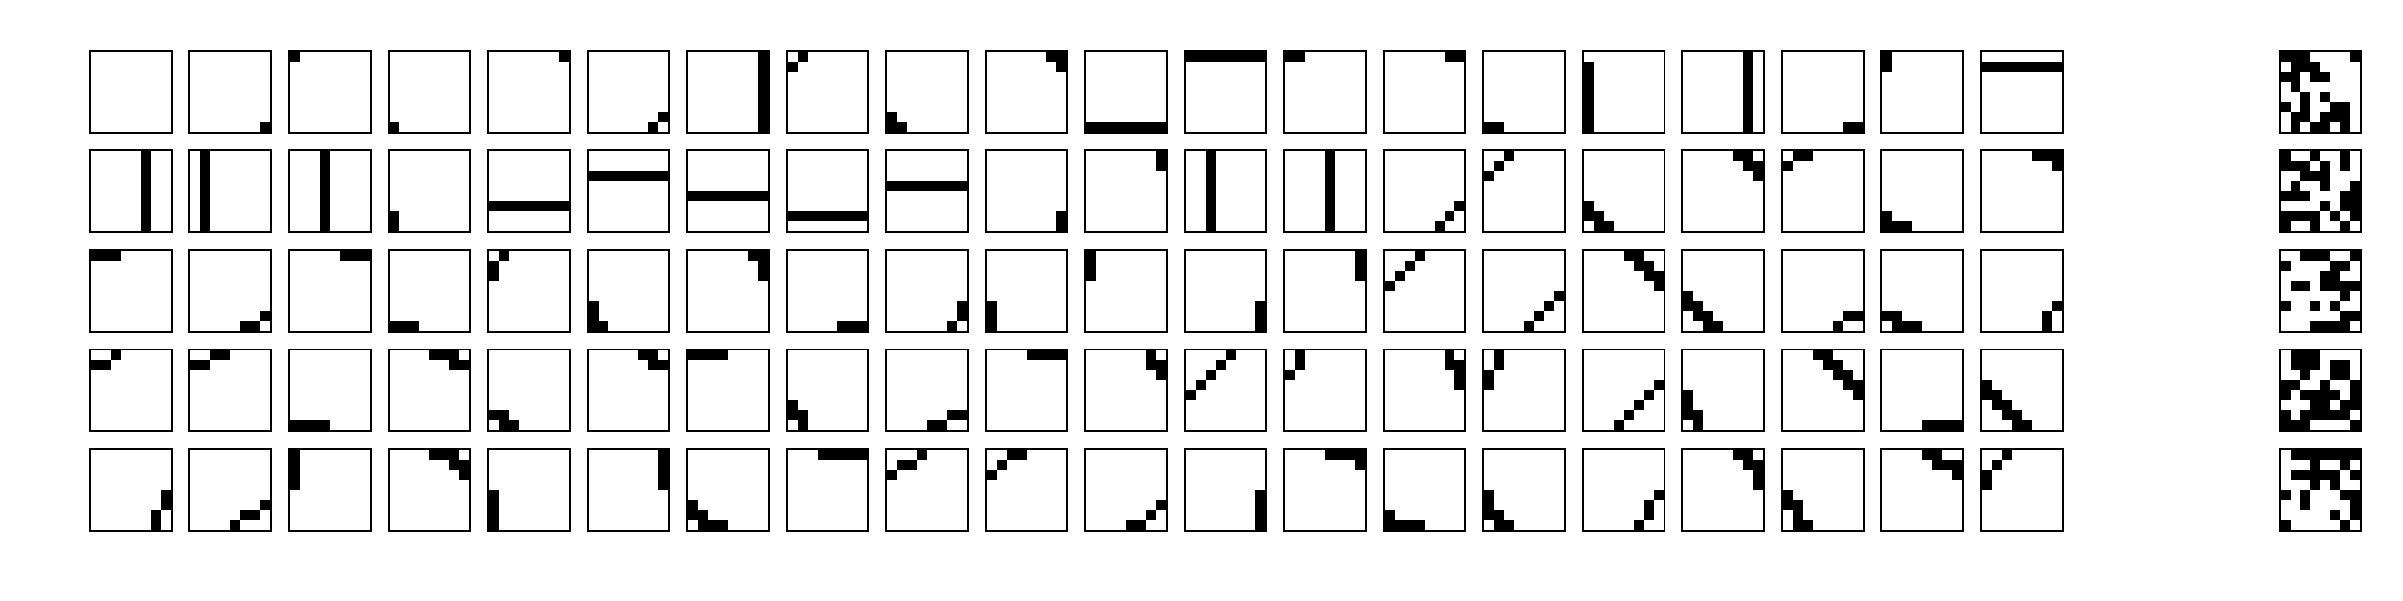
\includegraphics[width=\linewidth]{./gfx/window_values.pdf}
    \end{minipage}
  \end{center}
  \caption{The 100 most frequent windows accounting for approximately 82\% of the over 1.2 million $V_w$ values on a representative connectomics dataset contrasted with 5 randomly generated windows. Each box represents an 8 x 8 x 1 window where black pixels are boundary and white pixels are non-boundary.}
  \label{fig:bockwurst-frequency}
\end{figure}

Thus far, we have assumed the boundaries described in Section~\ref{sec:boundary-map} provide enough information to reconstruct the entire segmentation.
Pixels not on a segment boundary are easily relabeled using the $\texttt{Labels[]}$ array. 
However, more care is needed for pixels on the segment boundaries. 
Consider Figure~\ref{fig:bockwurst-encoding}, which depicts a difficult boundary to decode. 
If a boundary pixel has a non-boundary neighbor to the left or above, then that pixel merely takes on the value of that neighbor. 
However, the pixel $i$ requires more care since its relevant neighbors are both boundary pixels. 
If a non-boundary neighbor pixel shares a label with the undetermined pixel, we add the offset to that neighbor to an array \texttt{IndeterminateValues[]}. 
Otherwise we add that per-pixel label.
%\vspace{-1mm}
\paragraph{Metadata.}

We construct a data structure containing the two per-segment shape and two per-pixel label arrays. The last component of the data structure is the \texttt{Header}, which contains the dimensions of the original data, the window size, and the size of the arrays. \appName could be improved by further compressing the individual components of the encoding (e.g., Huffman encoding the $V_w$ values). We achieve strong overall compression by using a second-stage general compression scheme such as LZMA~(Sec.~\ref{sec:results}).


\subsection{Decoding}

The first step in decoding the data is to reconstruct the boundary map. We iterate over every pixel, determine the corresponding window $w$, and retrieve the encoded window value $f(V_w)$ from the $\texttt{WindowValues[]}$ array. These values range from $0$ to $N - 1$ and correspond to an index in $\texttt{ValueMapping[]}$ that contains the original $V_w$ value. After decoding $V_w$, the value of pixel $i$ in window $w$ equals $V_w \land 2^i$.

After reproducing the boundary map, we execute the same deterministic connected-components algorithm per slice as when encoding. Each component in the boundary map receives a label between $0$ and $M - 1$. Using the $\texttt{Labels[]}$ array, we can easily translate these component labels into the original per-pixel labels for every slice. To determine the per-pixel labels for every boundary pixel, we iterate over the entire dataset in raster order. Any boundary pixel $(x, y, z)$ with a non-boundary neighbor at $(x - 1, y, z)$ or $(x, y - 1, z)$ shares the same per-pixel label. If both relevant neighbors are boundaries we consider the next unused value in the $\texttt{IndeterminateValues[]}$ array and update this pixel's label.

\subsection{Complexity}

In what follows, $P$ is the number of input pixels; $N$ is the number of distinct window values; $X$, $Y$ and $Z$ are the size of the $x$, $y$, and $z$ dimensions of the input data;  and $\alpha$ is the inverse Ackermann function~\cite{fredman1989cell}.
%\vspace{-5mm}
\paragraph{Encoding.}

Extracting the boundaries from the segmentation, generating the $V_w$ values, and populating the $\texttt{IndeterminateValues[]}$ array are all linear work in $P$. The $N$ unique window values are sorted to create the $\texttt{ValueMapping}$ variable. Generating the $\texttt{Labels[]}$ array requires running a connected-component labeling algorithm over each $z$ slice; we use a union-find data structure with union by rank and path compression optimizations.  The overall complexity of the compression scheme is therefore $O\left({P(1 + \alpha(XY)) + N\log{N}}\right)$.
%\vspace{-5mm}
\paragraph{Decoding.}

Decoding the window values, reconstructing the boundary map, and applying the correct per-pixel labels for all boundary pixels using the array \texttt{IndeterminateValues[]} are all linear work in $P$.  Reconstructing the per-pixel labels requires running the connected-component labeling algorithm over every image slice. The overall complexity of the decompression scheme is therefore $O\left({P(1 + \alpha(XY))}\right)$.

%\subsection{Complexity}
%
%\paragraph{Encoding.}
%
%Extracting the boundaries from the segmentation and generating the $V_w$ values is linear in the number of input pixels $P$. The $N$ unique window values are sorted to create the $\texttt{ValueMapping}$ variable. Generating the $\texttt{IDs}$ array requires running a connected-component labeling algorithm over each $z$ slice. The algorithm uses a union-find data structure with union by rank and path compression optimizations. Populating the $\texttt{IndeterminateValues}$ array is linear in the number of pixels. With $X$, $Y$ and $Z$ as the size of the $x$, $y$, and $z$ dimensions of the input data, $N$ as the number of unique window values, and $P$ as the number of pixels, the complexity of the compression scheme is $O\left({P(1 + \alpha(XY)) + N\log{N}}\right)$, where $\alpha$ is the inverse Ackermann function\cite{Fredman:1989:CPC:73007.73040}.
%
%\paragraph{Decoding.}
%
%Decoding the window values and reconstructing the boundary map is linear in the number of input pixels $P$. Reconstructing the per-pixel labels requires running the connected-component labeling algorithm over every image slice. Applying the correct per-pixel labels for all boundary pixels using $\texttt{IndeterminateValues}$ is linear in the number of input pixels. With $X$ and $Y$ as the size of the $x$ and $y$ dimensions, and $P$ as the number of pixels, the complexity of the decompression scheme is $O\left({P(1 + \alpha(XY))}\right)$.


\section{Evaluation and Results} \label{sec:results}

%
%\paragraph{AC3 Subvolume.} For development and parameter exploration, we use the publicly-available dataset of mouse cortex known in the community as AC3. The dataset size is $1024\times1024\times75$ voxels and the resolution is $6\times6\times30~\text{nm}^3\text{/voxel}$. AC3 was acquired using serial section transmission electron microscopy (ssTEM).
%
%\paragraph{L. Cylinder.} We use the left part of the 3-cylinder mouse cortex volume of Kasthuri et al.~\cite{kasthuri2015saturated} ($2048\times2048\times50$ voxels). The tissue is dense mammalian neuropil from layers 4 and 5 of the S1 primary somatosensory cortex, acquired using serial section electron microscopy (ssEM). The dataset resolution is $3\times3\times30~\text{nm}^3\text{/voxel}$. Image data and a manually-labeled expert `ground truth' segmentation is publicly available\footnote{\scriptsize{\url{https://software.rc.fas.harvard.edu/lichtman/vast/}}}.
%
%\paragraph{CREMI.} As part of the MICCAI 2016 challenge on circuit reconstruction from electron microscopy images (CREMI), six ssTEM datasets were made publicly available\footnote{\scriptsize{\url{http://www.cremi.org}}},  each $1250\times1250\times125$ voxels. The volumes are part of an adult fruit fly (Drosophila melanogaster) brain. The resolution of all three datasets is $4\times4\times40~\text{nm}^3\text{/voxel}$. We include the CREMI A dataset for our evaluation.
%\\~\\
%We use a state-of-the-art method to create a dense automatic segmentation of the datasets.
%Membrane probabilities are generated using a convolutional neural network based on the U-net architecture~\cite{RonnebergerFB15}.
%The probabilities are used to seed watershed and generate an oversegmentation using superpixels.
%Agglomeration is then performed by the GALA active learning classifier~\cite{nunez2014graph}.
%The output of the agglomeration is shown in Fig.~\ref{fig:data}.
%
%\paragraph{MRI.} We include a label map of a T1-weighted brain MRI scan to evaluate compression on non-connectomics data. The dataset dimensions are $250\times250\times250$ voxels with a resolution of $1\times1\times1~\text{mm}^3\text{/voxel}$. This dataset is isotropic. The segmentation was obtained using the publicly available tool FreeSurfer\footnote{\scriptsize{FreeSurfer is available at \url{https://surfer.nmr.mgh.harvard.edu/}.}}.

%\subsection{Parameter Estimation}
%\paragraph{Varying Window Size.}
%\begin{figure}
%	\begin{center}
%		\includegraphics[width=0.7\textwidth]{./gfx/bockwurst_window_size.png}
%		\caption{The above plots show the effect of window size on the compression ratio. The left subplot shows the variation with window sizes $(n, n, 1)$ for $n$ ranging between $1$ and $720$. The right subplot shows the results where $z$ is no longer constrained to equal 1.}
%		\label{fig:bockwurst-window-size}
%	\end{center}
%\end{figure}
%Figure \ref{fig:bockwurst-window-size} shows the compression results of \appName on several connectomics datasets. There is a trade-off between the number of windows and the number of unique window values when varying the window size. The compression ratio generally peaks around the same window sizes across several different data sets.

We consider the following compression schemes: Compresso, Neuroglancer, Brotli, BZip2, Zlib, LZ78, LZF, LZMA, LZO, LZW, Zopfli, Zstandard, PNG, JPEG2000, and X.264. 
In addition to these stand-alone compression schemes we consider all pairs with a first stage encoding using either Compresso or Neuroglancer and a second stage using one of the general-purpose algorithms. 
Both \appName and Neuroglancer leave some redundancies that a general-purpose compressor can easily reduce; such multi-stage schemes are common in image compression. 
Table~\ref{tab:datasets} presents six connectomics, three MRI, and two image segmentation datasets used for evaluation. 
Compresso works for any arbitrary 2-D and 3-D window dimensions. We achieve the results in this section using an 8x8x1 window.

%We consider the following compression schemes: \appName, Neuroglancer, Run-Length Encoding (RLE), Brotli, BZip2, Zlib, LZ78, LZF, LZMA, LZO, LZW, Zopfli, Zstandard, PNG, JPEG2000, and X.264. In addition to these stand-alone compression schemes we consider all pairs between \appName, Neuroglancer, RLE, and the following general-purpose algorithms: Brotli, BZip2, ZLIB, LZ78, LZF, LZMA, LZO, LZW, Zopfli, Zstandard.

The combination of \appName and LZMA provides superior compression on all connectomics datasets (Tab.~\ref{tab:datasets}). Figure~\ref{fig:compression_ratios} shows the compression ratios for every compressor on segmentation data. For example, \appName achieves a compression ratio of over 950x on $L. Cylinder$ reducing the 10 gigabyte volume to 10.5 megabytes. LZMA performs very well by itself and paired with any encoding strategy. X.264 performs surprisingly poorly on these datasets, in part because

\begin{table}[!th]
\begin{minipage}{\textwidth}
\small
\caption{For evaluation, we use the following publicly available datasets. Segmentations were obtained using a combination of U-net~\cite{ronneberger2015u} and watershed, semi-automatic, or manually. Compresso paired with LZMA yields the best compression ratio on all datasets indicated by an asterisk (\textbf{*}). Neuroglancer paired with LZMA achieved the best compression ratio only for the SPL Brain Atlas (724x).}%While the training of our classifier is more expensive, testing accuracy is superior. }
\resizebox{\linewidth}{!}{
\begin{tabular}{l@{\hskip .1in}l@{\hskip .1in}l@{\hskip .2in}l@{\hskip .2in}l}
\toprule
Dataset & Size & Segmentation &  \multicolumn{2}{c}{\makecell{\textbf{Compresso} + \textbf{LZMA}\\Speed (Com./Dec.)~~~~~Compression Ratio}}\\
\midrule
\makecell[l]{\emph{AC3 Subvolume\footnotemark}\\~~mouse cortex, EM} & \makecell[l]{$1024\times1024\times150$ vx\\($6\times6\times30~\text{nm}^3\text{/vx}$)} & U-net & \makecell[l]{100 / 209 MB/s} & 814x \textbf{*}\\
\makecell[l]{\emph{AC4 Subvolume}\\~~mouse cortex, EM} & \makecell[l]{$1024\times1024\times100$ vx\\($6\times6\times30~\text{nm}^3\text{/vx}$)} & U-net & \makecell[l]{105 / 218 MB/s} & 701x \textbf{*}\\
\makecell[l]{\emph{L. Cylinder\footnotemark}~\cite{kasthuri2015saturated}\\~~mouse cortex, EM} & \makecell[l]{$2048\times2048\times300$ vx\\($3\times3\times30~\text{nm}^3\text{/vx}$)} & U-net & \makecell[l]{103 / 180 MB/s} & 952x \textbf{*}\\
\makecell[l]{\emph{CREMI A, B, C\footnotemark}\\~~drosophila brain, EM} & \makecell[l]{$1250\times1250\times125$ vx\\($4\times4\times40~\text{nm}^3\text{/vx}$)} & U-net & \makecell[l]{110 / 218, 118 / 243, \\ 110 / 219 MB/s} & \makecell[l]{857x \textbf{*}, 1239x \textbf{*}\\960x \textbf{*}}\\
\makecell[l]{\emph{SPL Brain Atlas\footnotemark}\\~~T1/T2-weighted MRIs} & \makecell[l]{$256\times256\times256$ vx\\($1\times1\times1~\text{mm}^3\text{/vx}$)} & Semi-autom. & \makecell[l]{85 / 254 MB/s} & 636x\\
\makecell[l]{\emph{SPL Knee Atlas\footnotemark}\\~~
MRI} & \makecell[l]{$512\times512\times119$ vx\\($0.277\times0.277\times1~\text{mm}^3\text{/vx}$)} & Semi-autom. & \makecell[l]{136 / 244 MB/s} & 1553x \textbf{*}\\
\makecell[l]{\emph{SPL Abdominal Atlas\footnotemark}\\~~CT} & \makecell[l]{$256\times256\times113$ vx\\($0.9375\times0.9375\times1.5~\text{mm}^3\text{/vx}$)} & Semi-autom. & \makecell[l]{91 / 254 MB/s} & 480x \textbf{*}\\
\makecell[l]{\emph{BSD500\footnotemark}\\~~Segmentation Challenge} & $321\times481$, 2696 images & Manual & \makecell[l]{110 / 187 MB/s} & 1188x \textbf{*}\\
\makecell[l]{\emph{PASCAL VOC\footnotemark}\\~~2012 Challenge } & Varying, 2913 images & Manual & \makecell[l]{146 / 222 MB/s} & 2217x \textbf{*}\\
\bottomrule
\end{tabular}
}
\label{tab:datasets}
\end{minipage}
\end{table}
\addtocounter{footnote}{-8} %3=n
\stepcounter{footnote}\footnotetext{\scriptsize{AC3+AC4 Subvolumes: \url{http://openconnecto.me/catmaid/?dataview=13}}}
\stepcounter{footnote}\footnotetext{\scriptsize{L. Cylinder: \url{https://software.rc.fas.harvard.edu/lichtman/vast/}}}
\stepcounter{footnote}\footnotetext{\scriptsize{CREMI A+B+C: \url{http://www.cremi.org}}}
\stepcounter{footnote}\footnotetext{\scriptsize{SPL Brain Atlas: \url{http://www.spl.harvard.edu/publications/item/view/2037}}}
\stepcounter{footnote}\footnotetext{\scriptsize{SPL Knee Atlas: \url{http://www.spl.harvard.edu/publications/item/view/1953}}}
\stepcounter{footnote}\footnotetext{\scriptsize{SPL Abdominal Atlas: \url{http://www.spl.harvard.edu/publications/item/view/1918}}}
\stepcounter{footnote}\footnotetext{\scriptsize{BSD500: \url{https://www.eecs.berkeley.edu/Research/Projects/CS/vision/grouping/resources.html}}}
\stepcounter{footnote}\footnotetext{\scriptsize{VOC2012: \url{http://host.robots.ox.ac.uk/pascal/VOC/voc2012/}}}

%\stepcounter{footnote}\footnotetext{\scriptsize{FreeSurfer is available at \url{https://surfer.nmr.mgh.harvard.edu/}.}}

\begin{figure}[h]
	\begin{center}
		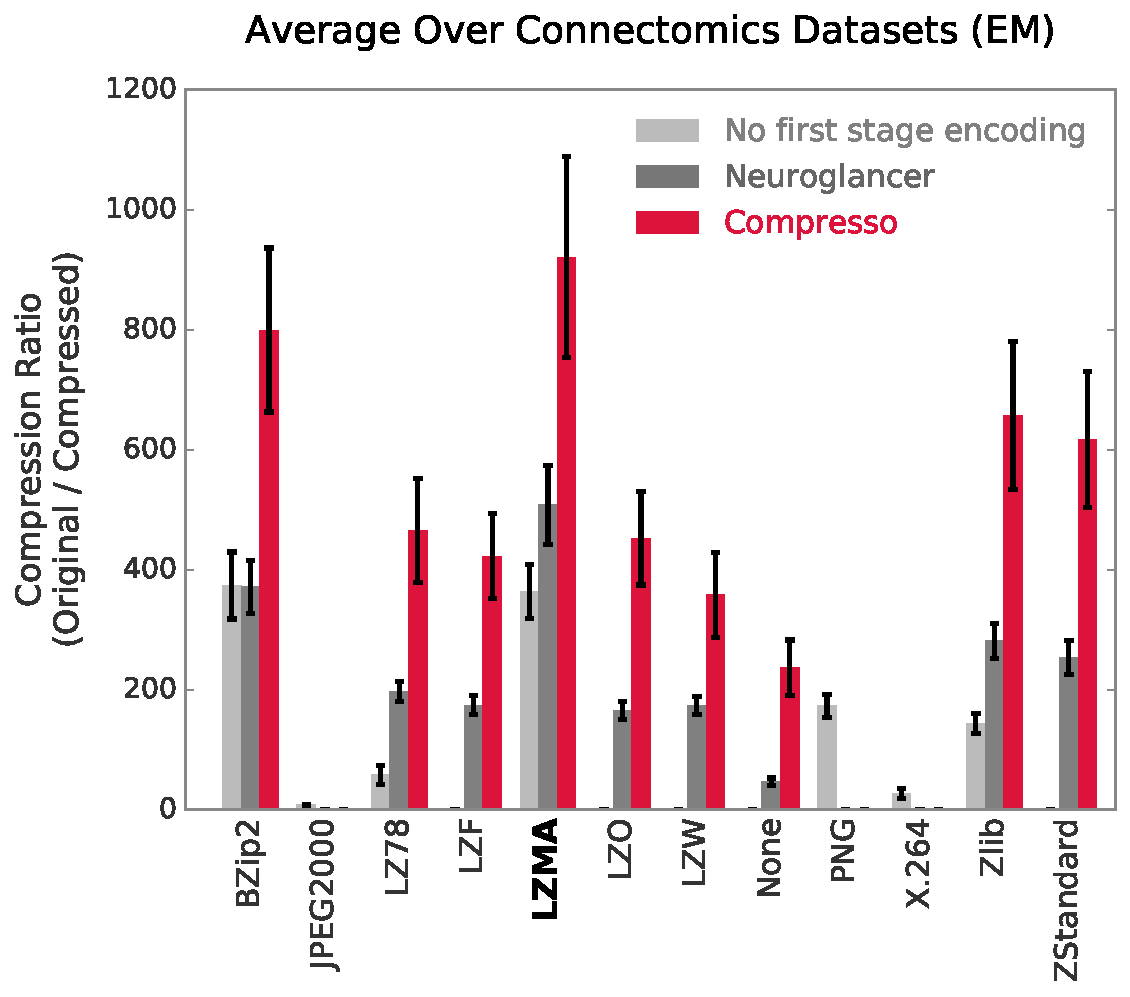
\includegraphics[width=0.5\textwidth]{gfx/LCylinder+ac3+ac4+cremiA+cremiB+cremiC_rhoana_compression_ratios.pdf}%
		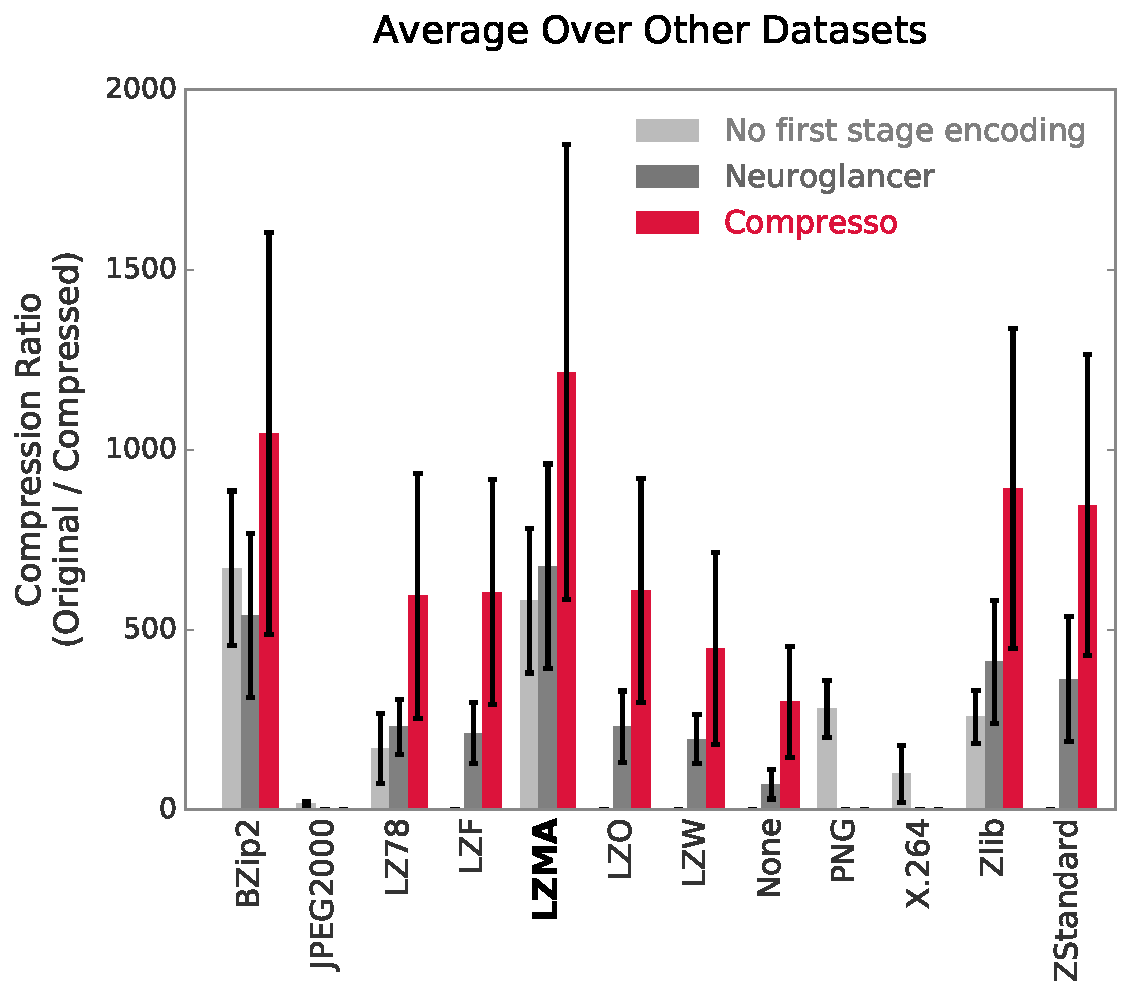
\includegraphics[width=0.5\textwidth]{gfx/VOC+mri1+mri2+mri3+BSD_gold_compression_ratios.pdf}%
		\caption{Compression ratios of general-purpose compression methods combined with \appName and Neuroglancer. % on all connectomics datasets (left) and on the other datasets (right).
%		the average on the remaining five connectomics datasets (right).
		\appName paired with LZMA yields the best compression ratios for all connectomics datasets and in average (four out of five) for the others.}
		\label{fig:compression_ratios}
	\end{center}
	\vspace{-18pt}
\end{figure}




%\vspace{-0.2cm}

\noindent of our requirement of lossless compression. It performs better when information loss is tolerated, however, even then it does not surpass the more specialized encoding schemes. These observations also hold for JPEG2000 and PNG. \appName with LZMA outperforms all other existing methods on connectomics datasets by 80\%. 

The fundamental principles guiding \appName are valid for a diverse set of segmentation datasets (Fig.~\ref{fig:compression_ratios}, right). We evaluate the performance of our compression scheme on three MRI and two image segmentation datasets to demonstrate additional potential use cases. \appName followed by LZMA compresses the MRI datasets reasonably well, particularly on the SPL Knee Atlas which contains highly redundant boundary segments.
%\appName followed by LZMA compresses the SPL Brain Atlas data by nearly a factor of 640x. 
The Berkeley Segmentation and PASCAL Visual Object Class datasets are two very common benchmarks in image segmentation~\cite{MartinFTM01,pascal-voc-2012}. Currently these datasets use GZIP and PNG compression but \appName with LZMA can improve on them by a factor of over 10x and 5x respectively. 

In terms of speed, \appName is on par with Neuroglancer across all datasets and achieves throughput of 112.16 megabytes per second ($SD = 18.62$ MB/s) for compression and 222.85 megabytes per second ($SD = 32.14$ MB/s) for decompression. All experiments ran on a single core of a Intel Xeon 2.3GHz CPU.

%Compared to all other methods, X.264 performs surprisingly poor on these datasets. Our requirement of lossless compression prevents this method from eliminating high frequencies between successive frames. We found that the video compression performs much better when information loss is tolerated. However, even then, the technique does not surpass the specialized encoding schemes discussed. These observations are also valid for JPEG2000 and PNG because of similar data assumptions.
 %The decompression speed for \appName was worse than the other encoding algorithms. However, there is significant room for optimization.


\section{Conclusions} \label{sec:c}
% Things we learned during this project, such as:
% - LZMA is black magic
% - Certain encodings do not necessarily lead to better results after compression but can significantly improve other properties such as compression speed or before compression space consumption
% - Mitzenmacher is a cool guy
% - etc.
%In this paper, we study and evaluate encoding and compression methods for segmentation data with focus on connectomics.
%
%%% Summary
%In this paper, we study and evaluate compression of segmentation data for connectomics and introduce \appName---an efficient compression tool that outperforms existing solutions.
%Interestingly, we have learned that simple encoding schemes (e.g., RLE) can perform existing methods already and that complexity does not always proof beneficial. \cf{Since we have removed RLE from the plot we need to make sure to name it somewhere briefly in the results!}
%
%%% Future work
%Besides connectomics datasets, we show that \appName efficiently compresses labeled brain MRI data and we believe it generalizes well on any kind of labeled segmentation data.
%In the future we plan to improve random access to lower memory requirements for online viewers and focus on more efficient compression of the metadata (Sec. ~\ref{sec:m}).
%Also, we will integrate \appName into our analysis pipeline and provide wrappers for various other clients.
%
%%% Promotion
%To encourage testing of our tool, replication of our experiments, and adoption in the community, we provide \appName and results as free and open research at (link omitted for review).%\appUrl.
We have introduced \appName, an efficient compression tool for segmentation data that outperforms existing solutions on connectomics, MRI, and other segmentation data. 
%We believe our approach will generalize well to other kinds of label data. 
In the future we plan to improve random access to lower memory requirements for online viewers and enhance compression of the metadata.
Also, we will integrate \appName into our analysis pipeline and various end-user applications. 
To encourage testing of our tool, replication of our experiments, and adoption in the community, we release \appName and our results as free and open research at \href{github.com/rhoana/Compresso}{github.com/rhoana/Compresso}. 
%{\color{White} B to the Ockwurst!}

\smallskip

{\small M. Mitzenmacher is supported in part by NSF grants CNS-1228598, CCF-1320231, CCF-1535795, and CCF-1563710. H. Pfister is supported in part by NSF grants IIS-1447344 and IIS-1607800, by the Intelligence Advanced Research Projects Activity (IARPA) via Department of Interior/Interior Business Center (DoI/IBC) contract number D16PC00002, and by the King Abdullah University of Science and Technology (KAUST) under Award No. OSR-2015-CCF-2533-01.}


%
% ---- Bibliography ----
%
\bibliographystyle{splncs03}
\bibliography{paper_references}

%\newpage
%\section{Appendix} \label{sec:appendix}

Additional Math:

TEMPORARY:

For example, we analyzed the proportion of windows encoded as a function of the $x$ most frequent values on the AC3 dataset with a window size of $8 \times 8 \times 1$. The most common $V_w$---corresponding to zero boundary pixels---accounts for nearly 75\% of all windows. The top 2,500 and 13,000 most common $V_w$ values include 90\% and 95\% of all windows respectively. If there are $|W|$ windows with $n$ bits each the expected number of unique values for a completely random boundary map (i.e. a pixel $p = 1$ with probability 0.5) is:

CONNECTED COMPONENT RESULTS:

For every image slice, the encoding uses a deterministic connected component algorithm. 
We define $M$ as the number of connected components $m \in [0, M)$. 
The identifier values themselves are not confined to this range but rather from $[0, 2^{64})$. 
We construct a function $g_z(m) \to [0, 2^{64})$ for every slice $z$ that maps a connected component index to its per-pixel identifier. 
Under this scheme, we transmit $64 * M$ bits per image slice to encode all of the per-pixel identifiers. 
In run-length encoding, an identifier is transmitted at least once for every x-scanline intersecting a given segment. 
On the AC3 dataset, using connected components instead of run-length encoding reduced the number of identifiers transmitted from 1,524,280 to 27,280 over 75 slices---a reduction of nearly 5,500\%. 







\begin{equation}
2^{n}\left[1 - \left(\frac{2^{n} - 1}{2^{n}}\right)^{|W|}\right]
\end{equation} 


Here we present additional plots for the CREMI, AC3 and MRI datasets.

%
%
%
\begin{figure}[h]
\includegraphics[width=0.5\textwidth]{gfx/cremi_enconly_bytes.pdf}%
\includegraphics[width=0.5\textwidth]{gfx/cremi_enconly_ratio.pdf}%
\\
\includegraphics[width=0.5\textwidth]{gfx/cremi_enconly_encodingspeed.pdf}%
\includegraphics[width=0.5\textwidth]{gfx/cremi_enconly_decodingspeed.pdf}%
\caption{Evaluation of encoding methods on the \textbf{CREMI} dataset. The Bockwurst encoding scheme (black) outperforms Neuroglancer and run-length encoding (RLE) in terms of compression ratio (top right) but decodes much slower (bottom right).}
\label{fig:cremi_encoding_results}
\end{figure}


\begin{figure}[h]
\includegraphics[width=0.5\textwidth]{gfx/cremi_compression_bytes.pdf}%
\includegraphics[width=0.5\textwidth]{gfx/cremi_compression_ratios.pdf}%
\\
\includegraphics[width=0.5\textwidth]{gfx/cremi_compression_total_comp_speed.pdf}%
\includegraphics[width=0.5\textwidth]{gfx/cremi_compression_total_decomp_speed.pdf}%
\caption{General-purpose compression methods with different encoding schemes on the \textbf{CREMI} segmentation data. A combination of Bockwurst encoding (red) and LZ78 yields the best performance (top right)---over $2\times$ higher compression ratio than any other method and $1600\times$ smaller than the uncompressed data.}
\label{fig:cremi_compression_results}
\end{figure}

%
%
%
\begin{figure}[h]
\includegraphics[width=0.5\textwidth]{gfx/ac3_enconly_bytes.pdf}%
\includegraphics[width=0.5\textwidth]{gfx/ac3_enconly_ratio.pdf}%
\\
\includegraphics[width=0.5\textwidth]{gfx/ac3_enconly_encodingspeed.pdf}%
\includegraphics[width=0.5\textwidth]{gfx/ac3_enconly_decodingspeed.pdf}%
\caption{Bockwurst performs best among the tested encoding methods on \textbf{AC3} which is also our training dataset (top right). While Bockwurst provides also a reasonable encoding speed (bottom left), the decoding performance is poor (bottom right).}
\label{fig:ac3_encoding_results}
\end{figure}


\begin{figure}[h]
\includegraphics[width=0.5\textwidth]{gfx/ac3_compression_bytes.pdf}%
\includegraphics[width=0.5\textwidth]{gfx/ac3_compression_ratios.pdf}%
\\
\includegraphics[width=0.5\textwidth]{gfx/ac3_compression_total_comp_speed.pdf}%
\includegraphics[width=0.5\textwidth]{gfx/ac3_compression_total_decomp_speed.pdf}%
\caption{Performance of general-purpose compression methods combined with run-length encoding (RLE), Neuroglancer and Bockwurst on the \textbf{AC3} connectomics dataset. Bockwurst encoding (red) with LZ78 results in a compression ratio of over $1400\times$. This is better than all other methods but the compression and decompression speeds leave room for optimization.}
\label{fig:ac3_compression_results}
\end{figure}


\begin{figure}[h]
\center
\includegraphics[width=0.5\textwidth]{gfx/mri.png}%
\caption{One slice of the \textbf{brain MRI} segmentation data with different anatomical parts labeled by a unique identifier and colored using a lookup table.}
\label{fig:mridata}
\end{figure}

%
% 
%
\begin{figure}[h]
\includegraphics[width=0.5\textwidth]{gfx/mri_enconly_bytes.pdf}%
\includegraphics[width=0.5\textwidth]{gfx/mri_enconly_ratio.pdf}%
\\
\includegraphics[width=0.5\textwidth]{gfx/mri_enconly_encodingspeed.pdf}%
\includegraphics[width=0.5\textwidth]{gfx/mri_enconly_decodingspeed.pdf}%
\caption{Evaluation of encoding methods on the labeled \textbf{brain MRI} dataset. Bockwurst encoding (black) yields less encoding performance than Neuroglancer but outperforms run-length encoding (RLE). The MRI data size is approximately 130 MB, resulting in 1-2 seconds encoding time using all methods. Bockwurst, however, is much slower in decoding.}
\label{fig:mri_encoding_results}
\end{figure}


\begin{figure}[h]
\includegraphics[width=0.5\textwidth]{gfx/mri_compression_bytes.pdf}%
\includegraphics[width=0.5\textwidth]{gfx/mri_compression_ratios.pdf}%
\\
\includegraphics[width=0.5\textwidth]{gfx/mri_compression_total_comp_speed.pdf}%
\includegraphics[width=0.5\textwidth]{gfx/mri_compression_total_decomp_speed.pdf}%
\caption{General-purpose compression methods with different encoding schemes on the labeled \textbf{brain MRI} data. A combination of Bockwurst encoding (red) and LZ78 yields the best performance.}
\label{fig:mri_compression_results}
\end{figure}


\end{document}
